\documentclass[aspectratio=169, 10pt]{beamer}

% ---- Theme ----
\usetheme{metropolis}

% ---- Packages ----
\usepackage{booktabs}
\usepackage{tikz}
\usetikzlibrary{shapes.geometric, arrows.meta, positioning, fit, backgrounds, calc}
\usepackage{listings}
\usepackage[T1]{fontenc}
\usepackage[sfdefault,scaled=.90]{FiraSans}
\usepackage{mathpazo}          % Palatino for serif family (\rmfamily)
\usepackage[utf8]{inputenc}
\usepackage{microtype}
\usepackage{array}
\usepackage{colortbl}
\usepackage{xcolor}
\usepackage{enumitem}
\usepackage{multirow}
\usepackage{pgfpages}
% To display notes on a second screen, uncomment one of:
% \setbeameroption{show notes on second screen=right}
% \setbeameroption{show notes}
\setbeamertemplate{note page}{\pagecolor{yellow!5}\insertnote}

% ---- Colors (Anthropic-inspired) ----
\definecolor{biokteal}{RGB}{35, 32, 28}           % warm deep charcoal
\definecolor{bioktorange}{RGB}{217, 119, 87}       % Anthropic coral orange
\definecolor{anthcream}{RGB}{250, 248, 245}        % warm cream
\definecolor{codebg}{RGB}{248, 246, 242}
\definecolor{codeframe}{RGB}{220, 212, 200}

% ---- Metropolis color overrides ----
\setbeamercolor{palette primary}{bg=biokteal, fg=white}
\setbeamercolor{progress bar}{fg=bioktorange, bg=bioktorange!20}
\setbeamercolor{title separator}{fg=bioktorange}
\setbeamercolor{frametitle}{bg=biokteal, fg=white}
\setbeamercolor{block title}{bg=biokteal!15, fg=biokteal}
\setbeamercolor{block body}{bg=biokteal!5}
\setbeamercolor{alerted text}{fg=bioktorange}
\setbeamercolor{normal text}{fg=biokteal}
\setbeamercolor{background canvas}{bg=anthcream}

\metroset{progressbar=frametitle, block=fill}

% ---- Typography: serif headings + sans-serif body ----
\setbeamerfont{title}{family=\rmfamily, series=\bfseries, size=\large}
\setbeamerfont{subtitle}{family=\rmfamily, shape=\itshape, size=\small}
\setbeamerfont{frametitle}{family=\rmfamily, series=\bfseries, size=\large}
\setbeamerfont{standout}{family=\rmfamily, series=\bfseries, size=\Large}
\setbeamerfont{author}{family=\rmfamily, size=\normalsize}
\setbeamerfont{institute}{family=\rmfamily, size=\small}

% ---- Symbol in footer of every slide ----
\setbeamertemplate{frame footer}{%
  \raisebox{1pt}{
\includegraphics[height=0.38cm]{claude_symbol.png}}%
}

% ---- Listings ----
\lstdefinestyle{biokt}{
  backgroundcolor=\color{codebg},
  basicstyle=\ttfamily\footnotesize,
  breaklines=true,
  frame=single,
  framerule=0.4pt,
  rulecolor=\color{codeframe},
  showstringspaces=false,
  tabsize=2,
  xleftmargin=4pt,
  xrightmargin=4pt,
}
\lstset{style=biokt}

% ---- TikZ node styles ----
\tikzset{
  tbox/.style={
    rectangle, rounded corners=3pt,
    draw=biokteal, fill=biokteal!12,
    text width=2.2cm, align=center,
    font=\small, inner sep=5pt, minimum height=0.7cm
  },
  wbox/.style={
    rectangle, rounded corners=3pt,
    draw=biokteal, fill=biokteal!20,
    text width=3.0cm, align=center,
    font=\small\bfseries, inner sep=6pt, minimum height=0.8cm
  },
  pbox/.style={
    rectangle, rounded corners=3pt,
    draw=bioktorange, fill=bioktorange!10,
    text width=2.4cm, align=center,
    font=\small, inner sep=5pt, minimum height=0.7cm
  },
  fbox/.style={
    rectangle, rounded corners=3pt,
    draw=biokteal, fill=biokteal!12,
    text width=3.6cm, align=center,
    font=\small, inner sep=5pt, minimum height=0.7cm
  },
  arr/.style={-Stealth, thick, color=biokteal!80},
  darr/.style={-Stealth, dashed, thick, color=gray!55},
  oarr/.style={-Stealth, thick, color=bioktorange},
}

% ---- Title info ----
\title{Claude Code for Biomolecular Simulation \& Computational Chemistry}
\subtitle{From First Principles to the BioKT Lab Configuration}
\author{David De Sancho}
\institute{University of the Basque Country (UPV/EHU) \& DIPC}
\date{\today}
\titlegraphic{
\includegraphics[height=1.2cm]{upvehu_logo_crop.pdf}\hfill
\includegraphics[height=0.8cm]{claude_logo_rsvg.pdf}}

% ============================================================
\begin{document}
% ============================================================

% ---- Slide 1: Title ----
\maketitle

% ============================================================
%   PART I: GENERAL CONCEPTS
% ============================================================

% ---- Prelude: Live Demo ----
\begin{frame}[standout]
  Prelude\\[0.4em]
  {\large Live Demo}
  \note{Before any slides: run the live demo. Open a terminal, navigate to the guanidinium project, and invoke \texttt{/dft-homo-lumo}. Let Claude read the skill, ask about the molecule, and generate the pipeline. Then switch to the Jupyter notebook to show the HOMO/LUMO orbital visualisation and the energy level diagram comparing guanidinium and guanidine. Expected time: 5--7 minutes. Then return to slides.}
\end{frame}

\begin{frame}{Prelude: \texttt{/dft-homo-lumo} on Guanidinium}
  \begin{columns}[T]
    \begin{column}{0.50\textwidth}
      \textbf{\color{biokteal}What just happened}
      \begin{itemize}[label=\textbullet]\setlength\itemsep{4pt}
        \item One prompt: molecule name and charge
        \item Claude read a skill file encoding the full protocol
        \item Generated 3D geometry $\to$ DFT optimisation $\to$ SCF
        \item Extracted HOMO/LUMO energies and cube files
        \item Notebook visualised the frontier orbitals
      \end{itemize}
    \end{column}
    \begin{column}{0.46\textwidth}
      \textbf{\color{biokteal}Key numbers}
      \renewcommand{\arraystretch}{1.3}
      \begin{tabular}{@{}lrr@{}}
        \toprule
        & \textbf{Guan.\ (+1)} & \textbf{Guan.\ (0)} \\
        \midrule
        HOMO (eV) & $-15.08$ & $-8.15$ \\
        LUMO (eV) & $-3.51$  & $+1.47$ \\
        Gap (eV)  & $11.57$  & $9.63$  \\
        \bottomrule
      \end{tabular}
      \vspace{0.5em}
      \begin{block}{}
        \small Method: CAM-B3LYP / def2-TZVP
      \end{block}
    \end{column}
  \end{columns}
  \note{This slide is a reference after the live demo --- it anchors the numbers and the method before moving on. The gap difference between the cation and neutral form (11.57 vs 9.63 eV) reflects the stabilisation of the LUMO by the positive charge. Use this to invite the audience's own chemical intuition before continuing.}
\end{frame}

% ---- Slide: Motivation ----
\begin{frame}{A Qualitative Shift in Research Practice}
  \begin{columns}[T]
    \begin{column}{0.48\textwidth}
      \begin{block}{The jagged frontier}
        \small AI is superhuman at some tasks and surprisingly poor at others. Knowing which is which requires genuine domain expertise --- not prompting skill.
      \end{block}
      \vspace{0.5em}
      \begin{block}{Expertise is rewarded, not replaced}
        \small The productivity gains from AI go disproportionately to those who already know their field deeply --- because they know when to trust the output and when to push back.
      \end{block}
    \end{column}
    \begin{column}{0.48\textwidth}
      \begin{block}{The bottleneck shifts}
        \small AI agents can work on many tasks in parallel. The limiting factor is no longer execution --- it is the quality of human judgment directing the work.
      \end{block}
      \vspace{0.5em}
      \begin{alertblock}{}
        \centering\small The tool does not determine the outcome.\\[0.2em] The expertise behind it does.
      \end{alertblock}
    \end{column}
  \end{columns}
  \note{The motivation for this talk is not hype. It is that the tools available to us now represent a genuine qualitative change in what a small research group can do -- but only if we use them wisely.\par
  The ``jagged frontier'' idea is important: AI is not uniformly capable. It can write a SLURM script faster than any of us, and it can also confidently produce a force field assignment that is subtly wrong. Recognising the difference requires domain expertise. This is why the tool rewards experts more than novices.\par
  The bottleneck shift is the deepest point. When execution is cheap, the value moves entirely to judgment: knowing what to ask, knowing what the answer should look like, knowing when something is wrong. That is exactly what a PhD or a postdoc should be developing.}
\end{frame}

% ---- Slide: Roadmap ----
\begin{frame}{Outline}
  \begin{columns}[T]
    \begin{column}{0.48\textwidth}
      \textbf{\color{biokteal}Part I --- General Concepts}
      \begin{itemize}[label=\textbullet]\setlength\itemsep{3pt}
        \item What Claude Code is (and is not)
        \item Installation, interfaces, operating modes
        \item \texttt{CLAUDE.md}, skills \& agents, memory, sessions
        \item Cost, privacy, and honest caveats
      \end{itemize}
      \vspace{0.7em}
      \textbf{\color{biokteal}Part II --- The BioKT Lab}
      \begin{itemize}[label=\textbullet]\setlength\itemsep{3pt}
        \item Scientific standards and compute infrastructure
        \item Skills library: QM, MD, enhanced sampling
        \item Daily workflow in practice
      \end{itemize}
    \end{column}
    \begin{column}{0.48\textwidth}
      \textbf{\color{biokteal}Closing}
      \begin{itemize}[label=\textbullet]\setlength\itemsep{3pt}
        \item What you can do starting Monday
        \item A caution on outsourcing judgment
      \end{itemize}
      \vspace{0.9em}
      \begin{block}{}
        \small Questions welcome throughout --- or at the end.
      \end{block}
    \end{column}
  \end{columns}
  \note{Give the audience the shape of the talk upfront. Part~I is about 15 minutes of general concepts -- useful to anyone using Claude Code, not just our lab. Part~II is lab-specific: the configuration, the skills library, and how it fits into a real research day. The demo comes at the end of Part~II. Allow 10 minutes for questions.}
\end{frame}

\begin{frame}[standout]
  Part I\\[0.4em]
  {\large General Concepts}
  \note{Introduce the two-part structure. Part~I covers general concepts that apply to any Claude Code user. Part~II shows how these are applied in the BioKT lab for biomolecular simulation. Estimated time: about 15 minutes for Part~I, 20 minutes for Part~II.}
\end{frame}

% ---- Slide 2: What Is Claude Code? ----
\begin{frame}{What Is Claude Code?}
  \begin{columns}[T]
    \begin{column}{0.49\textwidth}
      \textbf{\color{biokteal}What it IS}
      \begin{itemize}[label=\textbullet]\setlength\itemsep{4pt}
        \item An \alert{agentic AI coding assistant}
        \item Lives in your terminal or IDE
        \item Reads and writes files, runs shell commands
        \item Calls external tools and browses the web
        \item Operates in a loop: plan $\to$ act $\to$ observe \& validate
        \item Controlled by you at each step (or autonomously)
      \end{itemize}
    \end{column}
    \begin{column}{0.49\textwidth}
      \textbf{\color{biokteal}What it is NOT}
      \begin{itemize}[label=\textbullet]\setlength\itemsep{4pt}
        \item A chatbot (it \emph{does} things, not just talks)
        \item An autocomplete plugin
        \item A one-shot code generator
        \item A replacement for understanding your domain
      \end{itemize}
      \vspace{0.7em}
      \begin{block}{Key insight}
        You describe \emph{intent}; Claude figures out the steps, executes them, and reports back.
      \end{block}
    \end{column}
  \end{columns}
  \note{The key distinction from a chatbot: Claude Code has \textit{agency}. It does not just suggest -- it acts. It reads your directory structure, opens files, writes code, runs shell commands, and iterates on the results.\par
  The loop is: Claude proposes an action, waits for your approval (in default mode), executes it, reads the output, and decides what to do next. This continues until the task is complete.\par
  A useful mental model: a capable research assistant who can type at your keyboard. You describe what you need; it works out the steps.}
\end{frame}

% ---- Slide: Installation & VS Code Setup ----
\begin{frame}{Installation \& Setup}
  \begin{columns}[T]
    \begin{column}{0.48\textwidth}
      \textbf{\color{biokteal}Terminal (Mac / Linux)}
      \begin{itemize}[label=\textbullet]\setlength\itemsep{4pt}
        \item \alert{Install:}
              {\small\ttfamily curl -fsSL https://claude.ai/install.sh | bash}
        \item \alert{Launch \& auth:} \texttt{claude} --- browser opens for login
        \item Subscription or API key required
        \item Auto-updates in the background
      \end{itemize}
      \vspace{0.3em}
      {\small macOS alternative: \texttt{brew install -{}-cask claude-code}}
    \end{column}
    \begin{column}{0.48\textwidth}
      \textbf{\color{biokteal}VS Code Extension}
      \begin{itemize}[label=\textbullet]\setlength\itemsep{4pt}
        \item Extensions panel (\texttt{Ctrl+Shift+X})
        \item Search \textbf{Claude Code} --- publisher: Anthropic
        \item Provides: file tree, real-time diffs, inline edit review
      \end{itemize}
      \vspace{0.5em}
      \begin{block}{First steps after install}
        \small
        \begin{itemize}[label=\textbullet]\setlength\itemsep{2pt}
          \item Edit \texttt{{\raise.17ex\hbox{$\scriptstyle\sim$}}/.claude/CLAUDE.md} --- your standing brief
          \item Run \texttt{/init} inside a project to auto-generate a local \texttt{CLAUDE.md}
        \end{itemize}
      \end{block}
    \end{column}
  \end{columns}
  \note{Installation now requires no external dependencies -- a single \texttt{curl} command downloads and installs the \texttt{claude} CLI. The installer also sets up auto-updates in the background. On macOS, Homebrew is a clean alternative with \texttt{brew install --cask claude-code}.\par
  Running \texttt{claude} for the first time triggers browser-based OAuth against your Anthropic account -- no API key management needed. A Claude Pro, Max, Team, or Enterprise subscription is required.\par
  The VS Code extension is optional but lowers the barrier for users who want to see file diffs inline and navigate the project tree while Claude works. Both the CLI and extension share the same session and capabilities.\par
  After install, the first thing worth doing is writing a \texttt{CLAUDE.md} -- it is read every session and saves you from repeating context every time.}
\end{frame}

% ---- Slide: Cost & Privacy ----
\begin{frame}{Cost \& Privacy}
  \begin{columns}[T]
    \begin{column}{0.48\textwidth}
      \textbf{\color{biokteal}Cost}
      \begin{itemize}[label=\textbullet]\setlength\itemsep{4pt}
        \item \textbf{Claude Pro} --- {\raise.17ex\hbox{$\scriptstyle\sim$}}\$20/month; sufficient for most individual use
        \item \textbf{Claude Max} --- higher usage limits; better for heavy or autonomous workflows
        \item \textbf{API / Console} --- pay per token; useful for scripting and batch tasks
        \item No per-seat cost for the \texttt{claude} CLI itself
      \end{itemize}
    \end{column}
    \begin{column}{0.48\textwidth}
      \textbf{\color{biokteal}Privacy}
      \begin{itemize}[label=\textbullet]\setlength\itemsep{4pt}
        \item Anthropic does \textbf{not} use your conversations to train models by default
        \item Treat unpublished data with caution --- avoid pasting novel sequences, unreleased structures, or confidential results into the session
        \item Work with file paths and structure; minimise raw scientific data in the conversation window
      \end{itemize}
      \vspace{0.4em}
      \begin{alertblock}{\small Rule of thumb}
        \small Treat Claude as an unaffiliated third-party service: fine for published data, cautious for unpublished results, avoid for anything under IP protection or confidentiality obligations.
      \end{alertblock}
    \end{column}
  \end{columns}
  \note{Cost is a common question from PIs. Claude Pro at \$20/month is affordable for individual researchers and covers typical interactive use. Max plans make sense for users who run long autonomous sessions or heavy parallel workloads.\par
  Privacy is the more sensitive issue for a research lab. Anthropic's policy is that conversations are not used for training by default. But for unpublished science -- novel protein sequences, unreleased simulation data, results ahead of publication -- caution is warranted. The practical rule: work with file paths and let Claude read local files rather than pasting raw data into the chat.}
\end{frame}

% ---- Slide 3: Two Ways to Run ----
\begin{frame}{Two Ways to Run Claude Code}
  \begin{columns}[T]
    \begin{column}{0.46\textwidth}
      \centering
      \textbf{\color{biokteal}Terminal}\\[0.5em]
      \texttt{\$ claude}\\[0.4em]
      \begin{itemize}[label=\textbullet]\setlength\itemsep{4pt}
        \item Text-only interface
        \item Fast and lightweight
        \item Steeper initial barrier
        \item Ideal for scripting and quick tasks
      \end{itemize}
    \end{column}
    \begin{column}{0.02\textwidth}
      \textcolor{codeframe}{\rule{0.4pt}{5cm}}
    \end{column}
    \begin{column}{0.50\textwidth}
      \centering
      \textbf{\color{biokteal}IDE Extension (VS Code)}\\[0.5em]
      {\small Claude Code extension}\\[0.4em]
      \begin{itemize}[label=\textbullet]\setlength\itemsep{4pt}
        \item File tree and real-time diffs
        \item Review edits before accepting
        \item Lower barrier for new users
        \item Ideal for extended coding sessions
        \item Comfortable for remote work via SSH on different machines
      \end{itemize}
    \end{column}
  \end{columns}
  \note{Most researchers in this lab will use the terminal, since we are already comfortable there: just run \texttt{claude} in any directory.\par
  The VS~Code extension is useful for tasks where you want to see the file tree and review diffs inline before accepting. It is also a lower barrier for students new to the terminal.\par
  Both modes use the same API and have identical capabilities -- it is purely a question of interface preference. You can switch between them freely.}
\end{frame}

% ---- Slide 4: Four Operating Modes ----
\begin{frame}{Four Operating Modes}
  \begin{columns}[T]
    \begin{column}{0.24\textwidth}
      \begin{block}{Plan}
        \footnotesize
        \begin{itemize}[label=\textbullet]\setlength\itemsep{2pt}
          \item Read-only exploration
          \item No files are changed
          \item Think before acting
        \end{itemize}
      \end{block}
    \end{column}
    \begin{column}{0.24\textwidth}
      \begin{block}{Default}
        \footnotesize
        \begin{itemize}[label=\textbullet]\setlength\itemsep{2pt}
          \item Asks before every action
          \item Safest starting point
          \item Full control
        \end{itemize}
      \end{block}
    \end{column}
    \begin{column}{0.24\textwidth}
      \begin{block}{Accept Edits}
        \footnotesize
        \begin{itemize}[label=\textbullet]\setlength\itemsep{2pt}
          \item File edits auto-applied
          \item Shell commands still confirmed
          \item Good middle ground
        \end{itemize}
      \end{block}
    \end{column}
    \begin{column}{0.24\textwidth}
      \begin{block}{Auto}
        \footnotesize
        \begin{itemize}[label=\textbullet]\setlength\itemsep{2pt}
          \item Fully autonomous
          \item Runs commands freely
          \item Fastest; use with care
        \end{itemize}
      \end{block}
    \end{column}
  \end{columns}
  \vspace{1.2em}
  \begin{center}
    \texttt{Shift+Tab} cycles between modes $\quad|\quad$ Start cautious, gain speed through trust
  \end{center}
  \note{Plan mode is perhaps the most underused but most valuable mode. Use it when you are not sure what Claude will do -- it can read your files, plan an approach, and show you what it would change, without modifying anything.\par
  Auto mode is fully autonomous: Claude runs commands and applies edits without asking. Use it for well-defined, low-risk tasks. Combined with a powerful prompt it can make many changes quickly.\par
  Default mode is where most work starts: Claude asks for approval before every action.\par
  Accept Edits is a useful middle ground: file edits are applied automatically but shell commands still require approval -- useful once you trust Claude's code changes but want oversight on what runs.\par
  The single most useful keyboard shortcut to know: \texttt{Shift+Tab} to cycle between modes.}
\end{frame}

% ---- Slide 5: CLAUDE.md ----
\begin{frame}{\texttt{CLAUDE.md} --- Your Instruction File}
  \begin{columns}[T]
    \begin{column}{0.46\textwidth}
      \textbf{\color{biokteal}What it is}
      \begin{itemize}[label=\textbullet]\setlength\itemsep{3pt}
        \item A Markdown file loaded into \emph{every} session
        \item The ``system prompt you write''
        \item Global: \texttt{{\raise.17ex\hbox{$\scriptstyle\sim$}}/.claude/CLAUDE.md}
        \item Local: \texttt{<project>/CLAUDE.md} (project-specific)
        \item Changes Claude's behaviour without touching the model
      \end{itemize}
      \vspace{0.5em}
      \begin{block}{}
        \small Each session begins with a fresh context window --- \texttt{CLAUDE.md} is how you carry knowledge across sessions.
      \end{block}
    \end{column}
    \begin{column}{0.52\textwidth}
      \textbf{\color{biokteal}What to put in it}
      \begin{itemize}[label=\textbullet]\setlength\itemsep{3pt}
        \item \textbf{Role \& identity} --- who you are, your domain
        \item \textbf{Standards} --- correctness rules, safety constraints
        \item \textbf{Work preferences} --- how to communicate, what to ask
        \item \textbf{Infrastructure} --- machines, paths, software stack
        \item \textbf{Skill catalogue} --- which \texttt{/skills} exist and when to use them
        \item \textbf{Project structure} --- layout, git conventions
      \end{itemize}
    \end{column}
  \end{columns}
  \note{CLAUDE.md is loaded automatically into every Claude session. Think of it as a standing brief: who you are, what you work on, what standards to follow, what tools are available.\par
  The global file (\textasciitilde/.claude/CLAUDE.md) applies everywhere. You can also place a project-specific CLAUDE.md at the root of any project; it is merged with the global one.\par
  Worth investing an hour writing a thorough one. The return on that investment is felt in every subsequent session: Claude does not ask basic questions about your setup, and applies your standards automatically without being reminded.}
\end{frame}

% ---- Slide 6: Skills & Slash Commands ----
\begin{frame}[fragile]{Skills \& Slash Commands}
  \begin{columns}[T]
    \begin{column}{0.53\textwidth}
      \textbf{\color{biokteal}What they are}
      \begin{itemize}[label=\textbullet]\setlength\itemsep{3pt}
        \item Reusable workflows stored as \texttt{SKILL.md} files
        \item Triggered by typing \texttt{/skill-name} in the prompt
        \item Claude reads the instructions and executes them
        \item Loaded at startup --- restart after adding new skills
      \end{itemize}
      \vspace{0.4em}
      \textbf{\color{biokteal}Scope}
      \begin{itemize}[label=\textbullet]\setlength\itemsep{3pt}\small
        \item \textbf{Global:} \texttt{{\raise.17ex\hbox{$\scriptstyle\sim$}}/.claude/skills/} --- everywhere
        \item \textbf{Local:} \texttt{.claude/skills/} --- project only; in git
      \end{itemize}
      \vspace{0.2em}
      {\scriptsize\color{biokteal!70} The BioKT library lives in the shared repo \texttt{{\raise.17ex\hbox{$\scriptstyle\sim$}}/Software/Claude/Skills-BIOKT}, symlinked into \texttt{{\raise.17ex\hbox{$\scriptstyle\sim$}}/.claude/skills/}.\par}
      \vspace{0.4em}
      {\small\color{biokteal!70} Not all \texttt{/commands} are skills --- \texttt{/clear}, \texttt{/compact}, \texttt{/help} are built-in CLI commands that execute directly, not through Claude.}
    \end{column}
    \begin{column}{0.44\textwidth}
      \textbf{\color{biokteal}Example}
      \begin{lstlisting}
# In the Claude prompt:
/review-plan

# Claude stress-tests your plan:
#  - Identifies blind spots
#  - Checks best practices
#  - Flags wishful thinking
#  - Proposes alternatives
      \end{lstlisting}
      \vspace{0.4em}
      \textbf{\color{biokteal}Why they matter}
      \begin{itemize}[label=\textbullet]\setlength\itemsep{3pt}
        \item Encode expertise \emph{once}, reuse forever
        \item Share across machines and team members
        \item Build a personalised AI toolkit
      \end{itemize}
    \end{column}
  \end{columns}
  \note{Skills are Markdown files that contain workflow instructions for Claude to follow. When you type \texttt{/review-plan}, Claude reads the corresponding SKILL.md and follows the protocol described in it.\par
  The example is deliberately general: \texttt{/review-plan} stress-tests any plan -- a simulation protocol, a grant application, an analysis strategy -- by applying structured expert critique. It is useful to anyone in the room regardless of field.\par
  Scope matters: global skills are available on every machine and shared via git; project-local skills live inside the project directory and are only loaded when Claude runs there. This allows project-specific protocols without polluting the global toolkit.\par
  Skills are loaded at startup -- restart Claude Code after adding a new one.}
\end{frame}

% ---- Slide: Writing a Skill ----
\begin{frame}[fragile]{Writing a Skill: Template Syntax}
  \begin{columns}[T]
    \begin{column}{0.52\textwidth}
\begin{lstlisting}
# ~/.claude/skills/my-skill.md

# Skill Name

One or two sentences describing what
this skill does and when to trigger it.

## Arguments

$ARGUMENTS can include:
- molecule name, charge, basis set

## Instructions

### Step 1: Read context
Check the current directory for
relevant input files.

### Step 2: Execute
Run the protocol, validating each step.

### Step 3: Output
Report results in this format:
...
\end{lstlisting}
    \end{column}
    \begin{column}{0.44\textwidth}
      \textbf{\color{biokteal}Key elements}
      \begin{itemize}[label=\textbullet]\setlength\itemsep{4pt}
        \item \textbf{No YAML frontmatter} --- plain Markdown
        \item \textbf{Description} --- 1--2 sentences at the top; Claude reads this to decide when to invoke it
        \item \textbf{\texttt{\$ARGUMENTS}} --- whatever the user types after \texttt{/skill-name}
        \item \textbf{Step sections} --- each \texttt{\#\#\# Step N} is a concrete action with clear output
      \end{itemize}
      \vspace{0.5em}
      \begin{block}{}
        \small Start simple; add steps iteratively as you test. One working step beats five broken ones.
      \end{block}
    \end{column}
  \end{columns}
  \note{Skills are plain Markdown -- no special format required beyond the structure shown. Claude reads the file top to bottom and follows the instructions.\par
  The description at the top is the most important part: it is what tells Claude (and you) when the skill should be triggered. Keep it specific.\par
  \texttt{\$ARGUMENTS} is replaced at runtime with whatever the user types after the skill name. For \texttt{/dft-homo-lumo guanidinium +1}, \texttt{\$ARGUMENTS} becomes ``guanidinium +1''. Skills that take no input can omit the Arguments section.\par
  The step structure is a guideline, not a requirement. For simple workflows you might have a single Instructions section. For complex protocols, numbered steps help Claude track progress and help you debug when something goes wrong.\par
  Practical advice: start with the simplest version that does something useful, test it on a real task, and add detail only where the output is insufficient.}
\end{frame}

% ---- Slide: Skills vs Agents ----
\begin{frame}{Skills vs.\ Agents}
  \begin{columns}[T]
    \begin{column}{0.46\textwidth}
      \begin{block}{Skills --- \texttt{{\raise.17ex\hbox{$\scriptstyle\sim$}}/.claude/skills/}}
        \small Run \emph{inside} the main conversation.
        \begin{itemize}[label=\textbullet]\setlength\itemsep{3pt}
          \item Full chat history available
          \item Interactive; back-and-forth with user
          \item Triggered by \texttt{/skill-name}
        \end{itemize}
        \vspace{0.3em}
        \textbf{Use when:} user input needed mid-task, or conversation context matters.
      \end{block}
    \end{column}
    \begin{column}{0.46\textwidth}
      \begin{block}{Agents --- \texttt{{\raise.17ex\hbox{$\scriptstyle\sim$}}/.claude/agents/}}
        \small Run in an \emph{isolated} context window.
        \begin{itemize}[label=\textbullet]\setlength\itemsep{3pt}
          \item No prior conversation; returns single result
          \item Autonomous; own model and tool list
          \item Can run in \alert{parallel}
        \end{itemize}
        \vspace{0.3em}
        \textbf{Use when:} independent evaluation, parallel workloads, or focused bounded tasks.
      \end{block}
    \end{column}
  \end{columns}
  \vspace{0.5em}
  \begin{center}
    \small\textit{Example:} \texttt{/bash-parallelize} spawns N parallel agents for N independent replicas or mutants.
  \end{center}
  \note{Skills and agents represent two fundamentally different execution models.\par
  Skills run in the main conversation and have access to everything: the full chat history, all tools, the current context. They are interactive -- Claude can ask questions and the user can redirect mid-task. Most of the BioKT library is implemented as skills.\par
  Agents are sandboxed. They launch in a fresh context window with no memory of the current conversation. They receive a task, execute it autonomously, and return a result. They can run in parallel -- this is what \texttt{/bash-parallelize} exploits.\par
  The key question when choosing: does this task need my input along the way, or can I describe it completely upfront and let it run? If the former: skill. If the latter: agent.}
\end{frame}

% ---- Slide: Writing an Agent ----
\begin{frame}[fragile]{Writing an Agent: Template Syntax}
  \begin{columns}[T]
    \begin{column}{0.52\textwidth}
\begin{lstlisting}
# ~/.claude/agents/check-protocol.md

---
name: check-protocol
description: >
  Review simulation setup files for
  physical consistency and completeness
model: sonnet
tools:
  - Read
  - Glob
  - Grep
---

You are an independent simulation
reviewer. Check the mdp files, topology,
and SLURM script in the project for:
- Thermostat/barostat mismatches
- Cutoff values outside best practice
- Missing or inconsistent parameters

Report findings as a numbered list.
Do not modify any files.
\end{lstlisting}
    \end{column}
    \begin{column}{0.44\textwidth}
      \textbf{\color{biokteal}YAML frontmatter}
      \begin{itemize}[label=\textbullet]\setlength\itemsep{4pt}
        \item \textbf{name} --- unique identifier
        \item \textbf{description} --- tells Claude when to invoke this agent
        \item \textbf{model} --- \texttt{sonnet} / \texttt{opus} / \texttt{haiku}
        \item \textbf{tools} --- restrict to what is needed; read-only for review tasks
      \end{itemize}
      \vspace{0.5em}
      \textbf{\color{biokteal}Body (plain text)}
      \begin{itemize}[label=\textbullet]\setlength\itemsep{3pt}
        \item Role description
        \item Specific checks or steps
        \item Output format
        \item Explicit scope limits
      \end{itemize}
    \end{column}
  \end{columns}
  \note{The agent file is a Markdown file with YAML frontmatter -- identical to a skill file in structure, but stored in \texttt{{\raise.17ex\hbox{$\scriptstyle\sim$}}/.claude/agents/} and loaded differently.\par
  \texttt{name} is the identifier. \texttt{description} matters: Claude uses it to decide whether to spawn this agent when asked to delegate a task. \texttt{model} lets you assign a cheaper model for review tasks that do not need full Opus capability -- Sonnet is the right choice for most review tasks. \texttt{tools} is the key safety feature: restricting to read-only tools (Read, Glob, Grep) prevents the agent from modifying files unexpectedly.\par
  The body is plain prose instructions. Always include: the agent's role (``you are an independent reviewer''), what specifically to check, how to format the output, and what NOT to do (``do not modify any files''). Clear scope limits are important -- an agent that is not told to stay read-only may not.\par
  In the BioKT lab context, review agents are useful for checking simulation protocols before submission -- catching errors that the person who set up the simulation might overlook precisely because they wrote it.}
\end{frame}

% ---- Slide 7: Memory System ----
\begin{frame}{Memory System}
  \begin{block}{What is memory?}
    \small Each Claude session starts from scratch --- it remembers nothing from previous conversations. The \textbf{memory system} solves this by writing persistent Markdown files that are loaded into every new session, carrying knowledge across conversations and machines.
  \end{block}
  \vspace{0.4em}
  \begin{columns}[T]
    \begin{column}{0.50\textwidth}
      \textbf{\color{biokteal}Four memory types}
      \medskip

      \renewcommand{\arraystretch}{1.2}
      \begin{tabular}{@{}ll@{}}
        \toprule
        \textbf{Type} & \textbf{Stores} \\
        \midrule
        \texttt{user}      & Role, expertise, preferences \\
        \texttt{feedback}  & Corrections \& confirmed approaches \\
        \texttt{project}   & Goals, deadlines, decisions \\
        \texttt{reference} & Where to find external resources \\
        \bottomrule
      \end{tabular}
    \end{column}
    \begin{column}{0.48\textwidth}
      \textbf{\color{biokteal}How it works}
      \begin{itemize}\setlength\itemsep{4pt}
        \item Files in \texttt{{\raise.17ex\hbox{$\scriptstyle\sim$}}/.claude/projects/*/memory/}
        \item \texttt{MEMORY.md} index loaded in every session
        \item Claude saves memories proactively and on request
        \item Prevents repeating the same corrections
        \item Cross-session and cross-machine continuity
      \end{itemize}
      \vspace{0.5em}
      \begin{block}{}
        \small\centering
        \textit{``Remember X''} $\to$ saved immediately.\\
        \textit{``Forget X''} $\to$ file removed.
      \end{block}
    \end{column}
  \end{columns}
  \note{Claude has no built-in memory -- each session starts from scratch. The memory system solves this by maintaining persistent files that are loaded into every session context.\par
  The four types cover different timescales: user memories capture preferences that never change; feedback memories record corrections so mistakes are not repeated; project memories track the current state of active work; reference memories point to where external information lives.\par
  The MEMORY.md index must stay concise (it is in every context window). Detailed content lives in individual memory files and is read on demand.\par
  Practical example: if you correct Claude about a force field choice, say ``remember this.'' It saves a feedback memory and will not make the same error next time.}
\end{frame}

% ---- Slide: Session Management ----
\begin{frame}{Session Management}
  \begin{block}{What is context?}
    \small\textbf{Context} is everything Claude can currently ``see'': the conversation history, file contents read, tool outputs, and loaded instructions (\texttt{CLAUDE.md}, memory). The model can only act on what is in context --- nothing else exists for it.
  \end{block}
  \vspace{0.4em}
  \begin{columns}[T]
    \begin{column}{0.48\textwidth}
      \textbf{\color{biokteal}Why it matters}
      \begin{itemize}[label=\textbullet]\setlength\itemsep{4pt}
        \item Sessions grow; model attention dilutes
        \item Longer session $\neq$ better outcome
        \item Each turn becomes more expensive over time
        \item Strategic breaks produce cleaner results
      \end{itemize}
      \vspace{0.5em}
      \begin{block}{Key principle}
        \small Compact at task boundaries --- not in a crisis.
      \end{block}
    \end{column}
    \begin{column}{0.48\textwidth}
      \textbf{\color{biokteal}Core commands}
      \begin{itemize}[label=\textbullet]\setlength\itemsep{5pt}
        \item \texttt{/compact <hint>} --- summarise \& continue\\
              {\small Hint tells Claude what to keep; be specific}
        \item \texttt{/clear} --- empty conversation, fresh start\\
              {\small Best for switching to an unrelated task}
        \item \texttt{/rewind} (\texttt{Esc Esc}) --- restore a prior state\\
              {\small Keep file edits but drop the discussion, or vice versa}
      \end{itemize}
    \end{column}
  \end{columns}
  \note{Context is the totality of what the model can see: conversation history, file reads, tool outputs, and loaded instructions. It has a hard upper limit (the context window, currently around 200\,000 tokens for Claude) and a softer attention limit: as more content accumulates, the model's focus dilutes and quality can degrade even before the limit is reached.\par
  This is why context management is not just a technical detail -- it directly affects the quality of Claude's reasoning about your project.\par
  \texttt{/compact <hint>} is the workhorse: it summarises the conversation so far and continues in the same session. The hint is critical -- without it, important details often disappear on long or branching work. Good hint: ``we are setting up NPT equilibration for system X; keep the mdp choices and the topology decisions.''\par
  \texttt{/clear} is for a genuine fresh start -- unrelated task, different project. No summary is kept.\par
  \texttt{/rewind} (\texttt{Esc Esc}) is a selective undo: you can keep file edits and drop a circular discussion, or keep the dialogue and retry a bad edit. Four restore options are available.\par
  In the BioKT setup, the PreCompact hook runs \texttt{/checkpoint save} automatically before compaction, so session state is always checkpointed.}
\end{frame}

% ---- Slide 8: Settings & Hooks ----
\begin{frame}[fragile]{Settings \& Hooks}
  \begin{columns}[T]
    \begin{column}{0.53\textwidth}
      \textbf{\color{biokteal}\texttt{settings.json} key options}
      \begin{itemize}\setlength\itemsep{3pt}
        \item \textbf{model} --- which Claude model to use\\
              {\small (\texttt{sonnet}, \texttt{opus}, \texttt{haiku})}
        \item \textbf{permissions.allow} --- commands that run without a confirmation prompt\\
        \item \textbf{hooks} --- shell prompts triggered on events\\
              {\small (e.g.\ \texttt{PreCompact}, \texttt{PostToolCall})}
        \item \textbf{statusLine} --- dynamic terminal status display
        \item \textbf{MCP servers} --- connect Claude to external tools\\
              {\small databases, APIs, local services; worth exploring once comfortable with the basics}
      \end{itemize}
      \vspace{0.4em}
      {\small Global: \texttt{{\raise.17ex\hbox{$\scriptstyle\sim$}}/.claude/settings.json} \\ Local: \texttt{settings.local.json}}
    \end{column}
    \begin{column}{0.44\textwidth}
      \textbf{\color{biokteal}Hook example}
      \begin{lstlisting}
"hooks": {
  "PreCompact": [{
    "type": "prompt",
    "prompt": "Run /checkpoint save
    to checkpoint the session
    before compaction."
  }]
}
      \end{lstlisting}
      \vspace{0.3em}
      {\small Before context is compressed, Claude automatically saves the session state.}
    \end{column}
  \end{columns}
  \note{The permissions allowlist is a significant quality-of-life improvement. Without it, every read-only operation -- \texttt{git status}, \texttt{ls}, \texttt{python --version} -- requires manual approval. Adding common safe commands to the allowlist means Claude can execute them without interrupting your flow.\par
  The model setting balances capability and cost. Sonnet is the default: faster and cheaper, suitable for most tasks. Opus is more capable for complex reasoning.\par
  The PreCompact hook shown here is one we use in the lab: when the context window fills, Claude automatically runs \texttt{/checkpoint save} to checkpoint the session state before compaction.\par
  \texttt{settings.local.json} provides machine-specific overrides -- useful when different machines need different permissions or paths.\par
  MCP (Model Context Protocol) is worth mentioning briefly. It allows Claude to connect to external tools and data sources -- a local database, a file server, a domain-specific API. We have not yet explored MCP in the lab, but it is a natural next step for more advanced integrations.}
\end{frame}

% ============================================================
%   PART II: BIOKT CONFIGURATION
% ============================================================

% ---- Slide: Limitations ----
\begin{frame}{Honest Caveats}
  \begin{columns}[T]
    \begin{column}{0.48\textwidth}
      \textbf{\color{biokteal}What Claude does well}
      \begin{itemize}[label=\textbullet]\setlength\itemsep{4pt}
        \item Routine, well-documented protocols
        \item Boilerplate code, file I/O, scripting
        \item Aggregating and restructuring information
        \item Catching obvious errors in structured output
      \end{itemize}
    \end{column}
    \begin{column}{0.48\textwidth}
      \textbf{\color{biokteal}Where it falls short}
      \begin{itemize}[label=\textbullet]\setlength\itemsep{4pt}
        \item Domain-specific edge cases with sparse training data
        \item Subtle physical reasoning (e.g.\ rare force field combinations, unusual collective variables)
        \item Knowledge of \emph{your} system, your history, your failures
        \item It can be \alert{confidently wrong}
      \end{itemize}
    \end{column}
  \end{columns}
  \vspace{0.6em}
  \begin{block}{The bottom line}
    \small Claude produces drafts. Validation is always your responsibility.
  \end{block}
  \note{The ``jagged frontier'' metaphor is useful here: Claude's capabilities are not uniformly distributed. It can outperform experts at some tasks and fail embarrassingly at others, often in ways that are hard to predict without domain knowledge.\par
  The most dangerous failure mode is confident incorrectness: Claude produces output that looks right, uses correct terminology, and contains a subtle error that only a domain expert would catch. This is why the lab's scientific standards mandate validation at every stage.\par
  Claude has no memory of your specific system. It does not know that your protein has a tricky disulphide bond, that a previous equilibration failed for a known reason, or that a particular collective variable caused instability. You hold that context; Claude does not.}
\end{frame}

\begin{frame}[standout]
  Part II\\[0.4em]
  {\large The BioKT Lab Configuration}
  \note{Now we look at the specific configuration used in the BioKT lab. Everything from here is directly applicable to our daily research workflow. The general concepts just covered -- CLAUDE.md, skills, memory, settings -- are all present; we will see how each is concretely implemented.}
\end{frame}

% ---- Slide 9: Setup at a Glance ----
\begin{frame}{BioKT Setup at a Glance}
  \begin{center}
  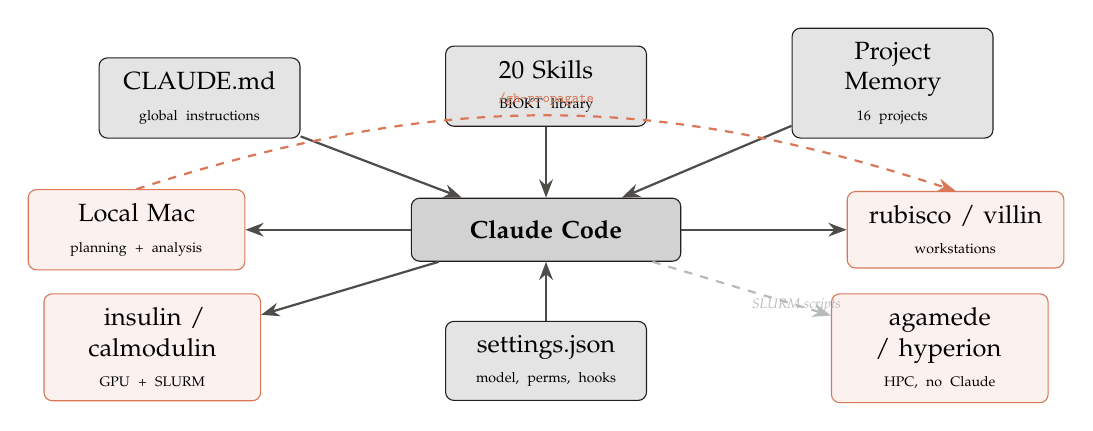
\begin{tikzpicture}[node distance=0.55cm and 0.9cm]
    \node[wbox] (cc) {Claude Code};

    \node[tbox, above left=0.75cm and 1.4cm of cc]  (cm)  {CLAUDE.md\\{\tiny global instructions}};
    \node[tbox, above=0.9cm of cc]                   (sk)  {20 Skills\\{\tiny BIOKT library}};
    \node[tbox, above right=0.75cm and 1.4cm of cc] (mem) {Project Memory\\{\tiny 16 projects}};
    \node[tbox, below=0.75cm of cc]                  (cfg) {settings.json\\{\tiny model, perms, hooks}};

    \node[pbox, left=2.1cm of cc]                   (mac) {Local Mac\\{\tiny planning + analysis}};
    \node[pbox, below left=0.4cm and 1.9cm of cc]   (gpu) {insulin / calmodulin\\{\tiny GPU + SLURM}};
    \node[pbox, right=2.1cm of cc]                  (ws)  {rubisco / villin\\{\tiny workstations}};
    \node[pbox, below right=0.4cm and 1.9cm of cc]  (hpc) {agamede / hyperion\\{\tiny HPC, no Claude}};

    \foreach \n in {cm, sk, mem, cfg}
      \draw[arr] (\n) -- (cc);
    \foreach \n in {mac, gpu, ws}
      \draw[arr] (cc) -- (\n);
    \draw[darr] (cc) -- (hpc) node[midway, below right, font=\tiny\itshape]{SLURM scripts};

    \draw[oarr, dashed, bend left=18]
      (mac.north) to node[above, font=\tiny\bfseries, color=bioktorange]{\texttt{/gh-propagate}} (ws.north);
  \end{tikzpicture}
  \end{center}
  \note{This diagram shows the full configuration. Claude Code runs on five interactive machines and is connected to four configuration layers: CLAUDE.md (global instructions), 20 skills (the BIOKT library), project memory (16 active research projects), and settings.json.\par
  The two HPC clusters -- agamede and hyperion -- do not have Claude installed because they use strict job scheduler policies. They receive SLURM scripts prepared by Claude on the interactive machines.\par
  \texttt{/gh-propagate} keeps everything in sync: update CLAUDE.md or add a skill on the Mac, and the change is pushed to a git repository and pulled on all other machines with a single command.}
\end{frame}

% ---- Slide 10: Scientific Standards ----
\begin{frame}{\texttt{CLAUDE.md}: Scientific Standards}
  \begin{center}
    {\large\bfseries\color{biokteal}``Correctness over speed''}\\[0.3em]
    {\small Simulation work goes on the scientific record --- a mistake found three steps later costs more than pausing to ask.}
  \end{center}
  \vspace{0.4em}
  \begin{columns}[T]
    \begin{column}{0.48\textwidth}
      \begin{itemize}\setlength\itemsep{5pt}
        \item[\textbf{1.}] \textbf{Ask rather than improvise}\\
              {\small Ambiguous parameter? Force field? Stop and ask.}
        \item[\textbf{2.}] \textbf{Validate before proceeding}\\
              {\small Check energy, $T$, $P$, RMSD after each stage.}
        \item[\textbf{3.}] \textbf{Never assume a prior step succeeded}\\
              {\small Check exit codes, log files, output files explicitly.}
      \end{itemize}
    \end{column}
    \begin{column}{0.48\textwidth}
      \begin{itemize}\setlength\itemsep{5pt}
        \item[\textbf{4.}] \textbf{Prefer known-good protocols}\\
              {\small No new flags without explanation and confirmation.}
        \item[\textbf{5.}] \textbf{Surface uncertainty explicitly}\\
              {\small Protonation state? Box size? Ion conc.? Say so.}
        \item[\textbf{6.}] \textbf{Errors and warnings are blockers}\\
              {\small Understand and resolve --- never suppress.}
      \end{itemize}
    \end{column}
  \end{columns}
  \note{This slide encodes the lab's scientific philosophy directly into CLAUDE.md. The ``correctness over speed'' principle is not a slogan -- it changes how Claude behaves in every session.\par
  Rule~1 is the most important: when there is ambiguity -- a protonation state, a force field version, a box size -- Claude stops and asks rather than picking a default silently. This prevents subtle errors that are hard to detect later.\par
  Rule~3 addresses chain failures: Claude checks exit codes, log files, and output files before proceeding. A GROMACS run that appears to finish but produced a corrupt trajectory is caught here.\par
  Rule~6: GROMACS notes and warnings may be benign, but they always need to be understood. Claude will not dismiss them without explanation.}
\end{frame}

% ---- Slide 11: Compute Infrastructure ----
\begin{frame}{Compute Infrastructure}
  \begin{center}
  \renewcommand{\arraystretch}{1.25}
  \begin{tabular}{@{}lllll@{}}
    \toprule
    \textbf{Host} & \textbf{Role} & \textbf{SLURM} & \textbf{GPU} & \textbf{Claude} \\
    \midrule
    \rowcolor{biokteal!10}
    local (Mac)  & Planning, analysis, writing & --- & ---  & \checkmark \\
    rubisco      & Remote workstation          & --- & yes  & \checkmark \\
    villin       & Remote workstation          & --- & yes  & \checkmark \\
    \rowcolor{biokteal!10}
    insulin      & GPU server                  & yes & yes  & \checkmark \\
    calmodulin   & GPU server (HP)             & yes & yes  & \checkmark \\
    \midrule
    \rowcolor{gray!12}
    agamede      & EHU HPC cluster             & yes & yes  & $\times$ \\
    \rowcolor{gray!12}
    hyperion     & DIPC HPC cluster            & yes & yes  & $\times$ \\
    \bottomrule
  \end{tabular}
  \end{center}
  \vspace{0.5em}
  \begin{itemize}
    \item \textbf{\texttt{/gh-propagate}} syncs \texttt{{\raise.17ex\hbox{$\scriptstyle\sim$}}/.claude} and \texttt{{\raise.17ex\hbox{$\scriptstyle\sim$}}/Software/Claude/Skills-BIOKT} to all \checkmark\ machines via git
    \item HPC clusters receive SLURM scripts prepared on interactive machines
  \end{itemize}
  \note{The table distinguishes two categories: interactive machines where Claude is installed, and HPC clusters where it is not.\par
  The local Mac is used for planning, analysis, and writing. It is the machine from which \texttt{/overview} runs -- it SSHes into all others to collect status.\par
  Rubisco and villin are remote workstations for lighter simulation work and development. Insulin and calmodulin are GPU servers running GROMACS with CUDA acceleration -- where most production simulations run.\par
  Agamede (EHU) and hyperion (DIPC) are external HPC systems accessed via SSH. Claude prepares SLURM scripts and input files on an interactive machine; you copy them and submit manually.\par
  \texttt{/gh-propagate} keeps the configuration synchronised across all five interactive machines.}
\end{frame}

% ---- Slide 12: Project Layout ----
\begin{frame}[fragile]{Standard Project Layout}
  \begin{columns}[T]
    \begin{column}{0.50\textwidth}
      \begin{lstlisting}
<ProjectName>/
|-- data/           # MD output (NOT git)
|   |-- *.xtc  *.gro  *.edr
|   `-- *.cpt  *.tpr  *.log
|-- analysis/
|   |-- notebooks/  # Jupyter (git)
|   `-- scripts/    # Python  (git)
|-- setup/          # mdp, top, itp, gro
|-- scripts/        # SLURM scripts
|-- README.md
`-- .gitignore
      \end{lstlisting}
    \end{column}
    \begin{column}{0.47\textwidth}
      \textbf{\color{biokteal}Key features}
      \begin{itemize}[label=\textbullet]\setlength\itemsep{4pt}
        \item \texttt{data/} excluded from git --- large binary files
        \item Analysis code tracked for reproducibility
        \item Same layout on \emph{all} machines --- predictable paths
        \item \texttt{new\_project.sh} scaffolds the tree and makes an initial commit
      \end{itemize}
      \vspace{0.5em}
      \begin{lstlisting}
# Create a new project:
~/Research/Projects/new_project.sh \
    MyProjectName
      \end{lstlisting}
    \end{column}
  \end{columns}
  \note{Consistent project layout is underrated. When every project follows the same structure across all machines, paths are predictable and Claude always knows where to look.\par
  The most important rule: \texttt{data/} is not in git. Raw MD output -- trajectories, restart files, energy files -- is often hundreds of gigabytes per project. The \texttt{.gitignore} handles exclusion automatically.\par
  What IS in git: analysis notebooks, Python scripts, mdp files, topology files, SLURM scripts. These define how the science was done and must be versioned.\par
  \texttt{new\_project.sh} scaffolds the directory tree, copies the standard \texttt{.gitignore}, initialises a git repository, and makes an initial commit. Starting a new project takes about ten seconds.}
\end{frame}

% ---- Slide 13: Skills Library ----
\begin{frame}{Skills Library: BioKT Collection}
  \begin{center}
  \renewcommand{\arraystretch}{1.05}
  {\scriptsize
  \begin{tabular}{@{}lll@{}}
    \toprule
    \textbf{Category} & \textbf{Skill} & \textbf{What it does} \\
    \midrule
    \multirow{2}{*}{Simulation prep}   & \texttt{/gmx-prep}           & GROMACS: EM $\to$ NVT $\to$ NPT $\to$ production \\
                                       & \texttt{/gmx-install}        & Build GROMACS + PLUMED from source \\
    \midrule
    \multirow{3}{*}{Enhanced sampling} & \texttt{/plumed-us}          & Umbrella sampling + WHAM \\
                                       & \texttt{/plumed-metad}       & Well-tempered metadynamics + sum\_hills \\
                                       & \texttt{/plumed-remd}        & US-REMD, bias-exchange, PT-METAD \\
    \midrule
    Parameterization                   & \texttt{/amber-parameterize} & SMILES $\to$ GAFF2 $\to$ GROMACS (.itp) \\
    Quantum chem.                      & \texttt{/dft-homo-lumo}      & PySCF DFT $\to$ HOMO/LUMO energies \\
    \midrule
    \multirow{4}{*}{Infrastructure}    & \texttt{/jobs}               & Track simulation jobs in JOBS.md \\
                                       & \texttt{/diy}                & Execute proposed commands / actions \\
                                       & \texttt{/sim-paths}          & SSH pre-flight file check \\
                                       & \texttt{/bash-parallelize}   & Parallel subagents for independent loops \\
    \midrule
    \multirow{4}{*}{Knowledge mgmt}   & \texttt{/overview}           & Aggregate TODO/CHECKPOINT across machines \\
                                       & \texttt{/checkpoint}               & Save/restore session context \\
                                       & \texttt{/bitacora}           & Append to lab notebook \\
                                       & \texttt{/tyler}              & PDF papers $\to$ markdown wiki \\
    \bottomrule
  \end{tabular}
  }
  \end{center}
  \note{This table shows a selection of the most-used BioKT skills; the full library has 20.\par
  Simulation prep -- \texttt{/gmx-prep} and \texttt{/gmx-install} -- form the foundation. These cover everything from building GROMACS from source to running a complete equilibration and production protocol.\par
  Enhanced sampling -- the three PLUMED skills -- cover our main methods for free energy calculations. Each suits different situations (discussed in detail on the next slides).\par
  Infrastructure skills solve real operational pain points: tracking jobs, verifying files before submission, and parallelising independent tasks.\par
  Knowledge management skills address a different problem: keeping research organised and recoverable across sessions and machines.\par
  Most lab members use \texttt{/gmx-prep} daily; infrastructure skills regularly; the PLUMED and QM skills are more project-specific.}
\end{frame}

% ---- Slide 14: gmx-prep ----
\begin{frame}{\texttt{/gmx-prep}: GROMACS MD Preparation}
  \begin{columns}[T]
    \begin{column}{0.50\textwidth}
      \textbf{\color{biokteal}Workflow stages}
      \vspace{0.4em}
      \begin{center}
      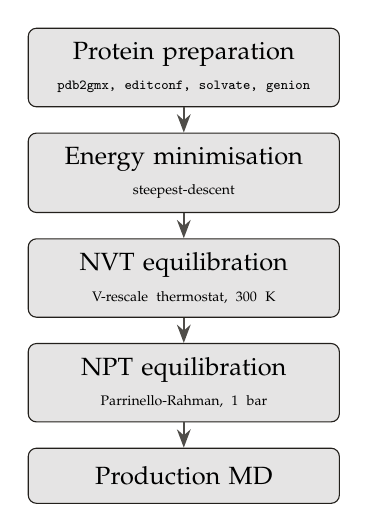
\begin{tikzpicture}[node distance=0.32cm]
        \node[fbox] (pp)  {Protein preparation\\{\tiny \texttt{pdb2gmx, editconf, solvate, genion}}};
        \node[fbox, below=of pp]  (em)  {Energy minimisation\\{\tiny steepest-descent}};
        \node[fbox, below=of em]  (nvt) {NVT equilibration\\{\tiny V-rescale thermostat, 300~K}};
        \node[fbox, below=of nvt] (npt) {NPT equilibration\\{\tiny Parrinello-Rahman, 1~bar}};
        \node[fbox, below=of npt] (md)  {Production MD};
        \draw[arr] (pp)--(em); \draw[arr] (em)--(nvt);
        \draw[arr] (nvt)--(npt); \draw[arr] (npt)--(md);
      \end{tikzpicture}
      \end{center}
    \end{column}
    \begin{column}{0.47\textwidth}
      \textbf{\color{biokteal}Default settings}
      \begin{itemize}\setlength\itemsep{3pt}
        \item Force field: \texttt{ff99SBws-STQ}
        \item Water model: \texttt{TIP4P/2005}
        \item Salt: 150~mM NaCl
        \item $T = 300$~K, $P = 1$~bar
        \item Timestep: 2~fs; cutoffs: 1.0~nm
        \item Electrostatics: PME
      \end{itemize}
      \vspace{0.5em}
      \textbf{\color{biokteal}Advanced options}
      \begin{itemize}\setlength\itemsep{3pt}
        \item AWH (free energy along a CV)
        \item H-REMD (Hamiltonian replica exchange)
        \item SLURM submission templates included
        \item Ligand integration via ACPYPE
      \end{itemize}
    \end{column}
  \end{columns}
  \note{This is the most frequently used skill in the lab.\par
  The workflow follows standard GROMACS best practices: prepare the protein topology, then minimise energy to relax clashes from the crystal structure, then equilibrate at constant volume (NVT) to reach the target temperature, then at constant pressure (NPT) to reach the target density, then run production.\par
  The default force field is ff99SBws-STQ -- a variant of AMBER99SB specifically optimised for intrinsically disordered proteins by Best and Mittal. It uses TIP4P/2005, currently the best-performing four-point water model for our systems.\par
  150~mM NaCl is standard physiological salt concentration.\par
  Advanced options: AWH for free energy calculations along a reaction coordinate; H-REMD for enhanced conformational sampling, particularly useful for disordered proteins.}
\end{frame}

% ---- Slide 15: Enhanced Sampling ----
\begin{frame}{Enhanced Sampling with PLUMED}
  \begin{columns}[T]
    \begin{column}{0.31\textwidth}
      \begin{block}{\texttt{/plumed-us}}
        \small
        \textbf{Umbrella Sampling}
        \begin{itemize}\setlength\itemsep{2pt}
          \item Harmonic restraint windows
          \item Serial or MPI/REMD execution
          \item WHAM free energy profile
          \item Bootstrap error estimation
          \item Convergence check (7 stages)
        \end{itemize}
      \end{block}
    \end{column}
    \begin{column}{0.31\textwidth}
      \begin{block}{\texttt{/plumed-metad}}
        \small
        \textbf{Well-Tempered MetaD}
        \begin{itemize}\setlength\itemsep{2pt}
          \item Adaptive Gaussian hills
          \item Biasfactor guidance
          \item \texttt{sum\_hills} FES
          \item Trajectory reweighting
          \item Block error analysis
        \end{itemize}
      \end{block}
    \end{column}
    \begin{column}{0.31\textwidth}
      \begin{block}{\texttt{/plumed-remd}}
        \small
        \textbf{Replica Exchange}
        \begin{itemize}\setlength\itemsep{2pt}
          \item US-REMD, bias-exchange
          \item PT-METAD temp.\ ladders
          \item \texttt{gmx\_mpi -multidir}
          \item Trajectory demultiplexing
          \item WHAM with weights
        \end{itemize}
      \end{block}
    \end{column}
  \end{columns}
  \vspace{0.7em}
  \begin{center}
    \small All three skills produce validated \texttt{plumed.dat} files, mdp modifications, and SLURM scripts.
  \end{center}
  \note{These three skills cover our main enhanced sampling methods, all using PLUMED as the biasing engine.\par
  \texttt{/plumed-us} is umbrella sampling: define windows along a collective variable, run independent simulations with harmonic restraints, combine with WHAM. Best when the CV is well defined and you want a clean free energy profile.\par
  \texttt{/plumed-metad} is well-tempered metadynamics: the bias is deposited adaptively as Gaussian hills, filling the free energy surface from below. Better for exploration when relevant regions are not known in advance.\par
  \texttt{/plumed-remd} adds replica exchange. US-REMD exchanges window configurations, accelerating convergence. Bias-exchange runs different CVs in different replicas. PT-METAD combines metadynamics with a temperature ladder.\par
  All three skills produce the \texttt{plumed.dat} file, mdp modifications, and the SLURM script ready to submit.}
\end{frame}

% ---- Slide 16: amber-parameterize ----
\begin{frame}{\texttt{/amber-parameterize}: Molecule Parameterization}
  \begin{columns}[T]
    \begin{column}{0.42\textwidth}
      \begin{center}
      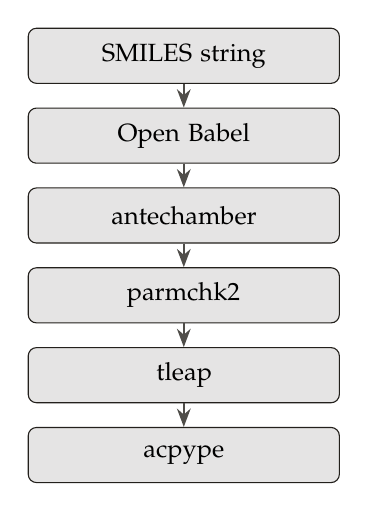
\begin{tikzpicture}[node distance=0.3cm]
        \node[fbox] (smi) {SMILES string};
        \node[fbox, below=of smi] (ob)  {Open Babel};
        \node[fbox, below=of ob]  (ant) {antechamber};
        \node[fbox, below=of ant] (par) {parmchk2};
        \node[fbox, below=of par] (tlp) {tleap};
        \node[fbox, below=of tlp] (acp) {acpype};
        \draw[arr] (smi)--(ob); \draw[arr] (ob)--(ant);
        \draw[arr] (ant)--(par); \draw[arr] (par)--(tlp);
        \draw[arr] (tlp)--(acp);
      \end{tikzpicture}
      \end{center}
    \end{column}
    \begin{column}{0.55\textwidth}
      \textbf{\color{biokteal}Key choices}
      \begin{itemize}\setlength\itemsep{4pt}
        \item Force field: \textbf{GAFF2} (General AMBER FF)
        \item Charges: \textbf{AM1-BCC} (default) or RESP
        \item Python wrapper automates the full pipeline
      \end{itemize}
      \vspace{0.5em}
      \textbf{\color{biokteal}Output \& integration}
      \begin{itemize}\setlength\itemsep{4pt}
        \item Output: \texttt{LIG.itp}, \texttt{LIG.gro} (GROMACS-ready)
        \item Integrates directly with \texttt{/gmx-prep}
        \item DFT-optimized geometries supported as input
        \item RDKit or Open Babel for initial 3D generation
      \end{itemize}
    \end{column}
  \end{columns}
  \note{This skill handles the common case of parameterising a small molecule -- a drug-like ligand, a cofactor, or a modified residue -- for use in a GROMACS simulation.\par
  The pipeline starts from a SMILES string: the standard compact notation for molecular structure. Open Babel generates a 3D geometry. Antechamber assigns GAFF2 atom types and calculates AM1-BCC partial charges. Parmchk2 finds missing parameters not in the GAFF2 database. Tleap assembles the AMBER topology. Acpype converts everything to GROMACS format.\par
  GAFF2 is the current standard general-purpose small-molecule force field for AMBER-family simulations. AM1-BCC charges are fast and accurate enough for most cases; RESP charges from a DFT calculation are available when higher accuracy is needed.\par
  The output files -- \texttt{LIG.itp} and \texttt{LIG.gro} -- plug directly into a topology prepared with \texttt{/gmx-prep}.}
\end{frame}

% ---- Slide 17: dft-homo-lumo ----
\begin{frame}{\texttt{/dft-homo-lumo}: Quantum Chemistry}
  \begin{columns}[T]
    \begin{column}{0.50\textwidth}
      \textbf{\color{biokteal}Pipeline}
      \vspace{0.4em}
      \begin{center}
      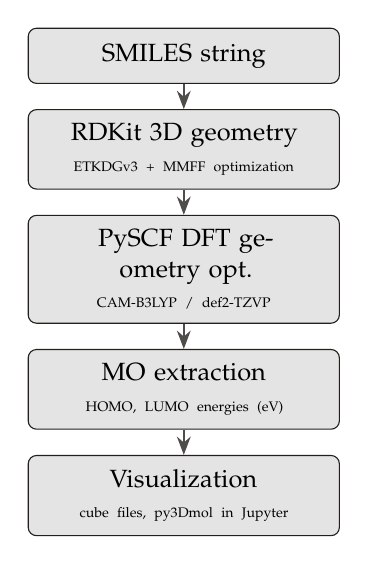
\begin{tikzpicture}[node distance=0.32cm]
        \node[fbox] (smi) {SMILES string};
        \node[fbox, below=of smi] (rdk) {RDKit 3D geometry\\{\tiny ETKDGv3 + MMFF optimization}};
        \node[fbox, below=of rdk] (dft) {PySCF DFT geometry opt.\\{\tiny CAM-B3LYP / def2-TZVP}};
        \node[fbox, below=of dft] (mo)  {MO extraction\\{\tiny HOMO, LUMO energies (eV)}};
        \node[fbox, below=of mo]  (vis) {Visualization\\{\tiny cube files, py3Dmol in Jupyter}};
        \draw[arr] (smi)--(rdk); \draw[arr] (rdk)--(dft);
        \draw[arr] (dft)--(mo); \draw[arr] (mo)--(vis);
      \end{tikzpicture}
      \end{center}
    \end{column}
    \begin{column}{0.47\textwidth}
      \textbf{\color{biokteal}Settings}
      \begin{itemize}\setlength\itemsep{3pt}
        \item Functional: \texttt{CAM-B3LYP}\\
              {\small alts: B3LYP, wB97X-D3, PBE0}
        \item Basis set: \texttt{def2-TZVP}\\
              {\small high-acc: \texttt{def2-QZVP}}
        \item Convergence: $10^{-6}$~Hartree
        \item Grid: level 4
      \end{itemize}
      \vspace{0.5em}
      \textbf{\color{biokteal}Integration}
      \begin{itemize}\setlength\itemsep{3pt}
        \item DFT-optimized geometry $\to$ \texttt{/amber-parameterize}
        \item RESP charges from DFT wavefunction
        \item Useful for metal-binding residues and cofactors
      \end{itemize}
    \end{column}
  \end{columns}
  \note{PySCF is a pure Python quantum chemistry package -- easy to install, no commercial licence required.\par
  CAM-B3LYP is a range-separated hybrid functional: it performs better than standard B3LYP for charge-transfer states and molecules with extended pi systems. def2-TZVP is a reliable triple-zeta basis for most organic molecules.\par
  Main use cases in the lab: characterising metal-binding cofactors or drug-like ligands, and providing higher-quality starting geometries and charges for the parameterisation pipeline.\par
  Integration with \texttt{/amber-parameterize}: the DFT-optimised geometry can replace the Open Babel geometry as input, and RESP charges derived from the wavefunction provide higher accuracy than AM1-BCC when needed.\par
  The cube files produced can be visualised directly in a Jupyter notebook using py3Dmol.}
\end{frame}

% ---- Slide 18: Workflow Infrastructure ----
\begin{frame}{Workflow Infrastructure}
  \begin{columns}[T]
    \begin{column}{0.31\textwidth}
      \begin{block}{\texttt{/jobs}}
        \small
        Maintains \texttt{JOBS.md} --- a table of all running and completed simulations across every machine.
        \begin{itemize}[label=\textbullet]\setlength\itemsep{2pt}
          \item Job name, machine, SLURM ID
          \item Start date, status, notes
          \item Archive completed jobs
        \end{itemize}
      \end{block}
    \end{column}
    \begin{column}{0.31\textwidth}
      \begin{block}{\texttt{/sim-paths}}
        \small
        SSH pre-flight check before job submission.
        \begin{itemize}[label=\textbullet]\setlength\itemsep{2pt}
          \item Verifies all required files exist on the target machine
          \item Checks .gro, .top, .mdp, .dat, .sh
          \item Catches missing files before queue wait
        \end{itemize}
      \end{block}
    \end{column}
    \begin{column}{0.31\textwidth}
      \begin{block}{\texttt{/bash-parallelize}}
        \small
        Spawns parallel subagents for independent tasks.
        \begin{itemize}[label=\textbullet]\setlength\itemsep{2pt}
          \item Detects independence in bash loops
          \item Load-aware concurrency control
          \item Collects and reports results
        \end{itemize}
      \end{block}
    \end{column}
  \end{columns}
  \vspace{0.7em}
  \begin{center}
    \small Example: analyse 8 replicas in parallel instead of sequentially with a single \texttt{/bash-parallelize} call.
  \end{center}
  \note{These three skills address operational problems that arise when managing many simulations across multiple machines.\par
  \texttt{/jobs} maintains a JOBS.md table in the project root. Every time a job is submitted, an entry is added; every time you check status, it is updated. Over time this gives a complete record of what ran, on which machine, with what outcome.\par
  \texttt{/sim-paths} does a pre-submission check: it SSHes to the target machine and verifies that all required input files actually exist. This catches the common mistake of forgetting to copy a file before submitting, which wastes queue time on the HPC clusters.\par
  \texttt{/bash-parallelize} is the most powerful of the three. When you have a bash loop running the same analysis on N independent systems -- 8 replicas, 12 mutants -- it converts the loop into N parallel Claude subagents. The speedup for analysis tasks can be substantial.}
\end{frame}

% ---- Slide 19: Knowledge Management ----
\begin{frame}{Knowledge \& Session Management}
  \begin{columns}[T]
    \begin{column}{0.48\textwidth}
      \begin{block}{\texttt{/overview}}
        \small Aggregates \texttt{CHECKPOINT.md} and \texttt{TODO.md} from all interactive machines via SSH. Produces a prioritised action plan for the day or week. Run from the local Mac.
      \end{block}
      \vspace{0.5em}
      \begin{block}{\texttt{/checkpoint save} / \texttt{load}}
        \small Checkpoints the current session state to \texttt{CHECKPOINT.md}. Run before \texttt{/clear} to avoid losing context. Restored automatically at next session start if the file is present in the project directory.
      \end{block}
    \end{column}
    \begin{column}{0.48\textwidth}
      \begin{block}{\texttt{/bitacora}}
        \small Appends a structured entry to \texttt{LABNOTEBOOK.md}: summary, decisions made, files touched, figures, next steps. Run before \texttt{/clear} to capture the session's scientific record.
      \end{block}
      \vspace{0.5em}
      \begin{block}{\texttt{/tyler}}
        \small Converts a folder of PDF papers into a two-tier markdown wiki: an \texttt{index.md} (${\sim}400$~tokens/paper) and per-paper \texttt{papers/*.md} files read on demand. Keeps literature accessible within Claude's context window.
      \end{block}
    \end{column}
  \end{columns}
  \note{These four skills address a different problem: keeping research organised and recoverable across sessions and machines.\par
  \texttt{/overview} is the morning routine. Run it from the local Mac; it SSHes into all interactive machines, reads their CHECKPOINT.md and TODO.md files, and produces a single prioritised action plan. It answers ``what should I work on today?'' across the whole infrastructure.\par
  \texttt{/checkpoint save} and \texttt{load} address the ephemeral nature of Claude sessions. \texttt{/checkpoint save} writes a session summary to CHECKPOINT.md. Running \texttt{/checkpoint load} at the next session start restores that context. The PreCompact hook triggers \texttt{/checkpoint save} automatically when the context window fills.\par
  \texttt{/bitacora} maintains LABNOTEBOOK.md -- a chronological record of what was done, what decisions were made, and what the next steps are.\par
  \texttt{/tyler} converts PDFs into a token-efficient markdown wiki, making your literature accessible to Claude without pasting full-text content.}
\end{frame}

% ---- Slide 20: A Day in the Lab ----
\begin{frame}{A Day in the Lab}
  \begin{center}
  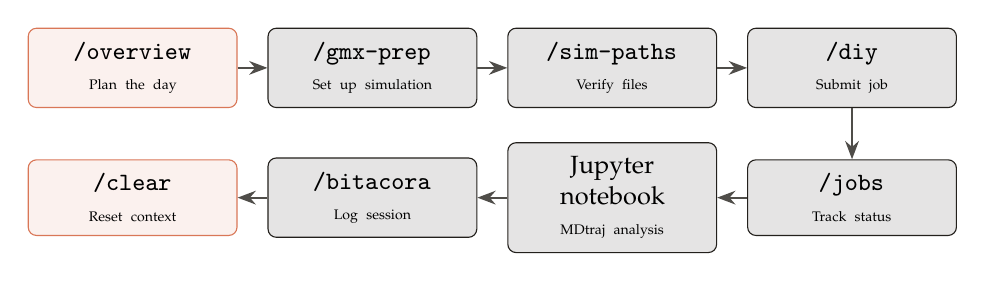
\begin{tikzpicture}[node distance=0.28cm and 0.32cm]
    \node[pbox, text width=2.3cm] (ov) {\texttt{/overview}\\{\tiny Plan the day}};
    \node[tbox, text width=2.3cm, right=0.38cm of ov]  (gp) {\texttt{/gmx-prep}\\{\tiny Set up simulation}};
    \node[tbox, text width=2.3cm, right=0.38cm of gp]  (sp) {\texttt{/sim-paths}\\{\tiny Verify files}};
    \node[tbox, text width=2.3cm, right=0.38cm of sp]  (dy) {\texttt{/diy}\\{\tiny Submit job}};

    \node[tbox, text width=2.3cm, below=0.65cm of dy]  (jb) {\texttt{/jobs}\\{\tiny Track status}};
    \node[tbox, text width=2.3cm, left=0.38cm of jb]   (nb) {Jupyter notebook\\{\tiny MDtraj analysis}};
    \node[tbox, text width=2.3cm, left=0.38cm of nb]   (bt) {\texttt{/bitacora}\\{\tiny Log session}};
    \node[pbox, text width=2.3cm, left=0.38cm of bt]   (cl) {\texttt{/clear}\\{\tiny Reset context}};

    \draw[arr] (ov)--(gp); \draw[arr] (gp)--(sp);
    \draw[arr] (sp)--(dy); \draw[arr] (dy)--(jb);
    \draw[arr] (jb)--(nb); \draw[arr] (nb)--(bt);
    \draw[arr] (bt)--(cl);
  \end{tikzpicture}
  \end{center}
  \vspace{0.4em}
  \begin{itemize}\setlength\itemsep{2pt}
    \item \textbf{Morning:} \texttt{/overview} reveals what is running and what needs attention
    \item \textbf{Setup:} Claude writes mdp files, prepares topology, generates SLURM script
    \item \textbf{Submit:} \texttt{/diy} executes proposed commands; \texttt{/jobs} records the new entry
    \item \textbf{Analyse:} notebooks with MDtraj, numpy, pandas --- Claude helps debug and extend
    \item \textbf{End of session:} \texttt{/bitacora} captures decisions; \texttt{/checkpoint save}; then \texttt{/clear}
  \end{itemize}
  \note{This slide shows how all the components work together in a typical day.\par
  Morning: \texttt{/overview} gives situational awareness -- what finished overnight, what is still running, what failed. You can plan the day without opening multiple SSH sessions.\par
  Setup: you ask Claude to prepare a new simulation. It asks clarifying questions, writes the mdp files, prepares the topology, and generates a SLURM submission script. Nothing is submitted yet.\par
  Verify: \texttt{/sim-paths} SSHes to the target machine and confirms all required files are present. If anything is missing, it reports exactly what and where.\par
  Submit and track: \texttt{/diy} executes the proposed submission command. \texttt{/jobs} records the new job in JOBS.md.\par
  End of session: \texttt{/bitacora} appends an entry to LABNOTEBOOK.md capturing what was done. \texttt{/checkpoint save} checkpoints the context. \texttt{/clear} resets the window ready for the next task.\par
  This workflow makes research more organised and reproducible -- without changing the fundamental way we do science.}
\end{frame}

% ---- Slide: Takeaways ----
\begin{frame}{What You Can Do Starting Monday}
  \begin{columns}[T]
    \begin{column}{0.48\textwidth}
      \textbf{\color{biokteal}First steps}
      \begin{itemize}[label=\textbullet]\setlength\itemsep{4pt}
        \item Install: {\small\ttfamily curl -fsSL https://claude.ai/install.sh | bash}
        \item Write your \texttt{CLAUDE.md} --- role, standards, infrastructure
        \item Run \texttt{/init} in one project to get a local \texttt{CLAUDE.md}
        \item Try \texttt{/dft-homo-lumo} on a molecule you know well
      \end{itemize}
    \end{column}
    \begin{column}{0.48\textwidth}
      \textbf{\color{biokteal}Build from there}
      \begin{itemize}[label=\textbullet]\setlength\itemsep{4pt}
        \item Use \texttt{/gmx-prep} for your next simulation setup
        \item Run \texttt{/overview} each morning to track active work
        \item End sessions with \texttt{/bitacora} and \texttt{/checkpoint save}
        \item Add skills as your workflows mature
      \end{itemize}
      \vspace{0.5em}
      \begin{block}{}
        \small Start with tasks you already know how to do. That way you can tell when Claude gets it right --- and when it does not.
      \end{block}
    \end{column}
  \end{columns}
  \note{The key message here is sequencing. Do not start with the most complex or unfamiliar task. Start with something routine -- a simulation setup, an analysis notebook -- where you already know what the output should look like. That gives you the ground truth to evaluate Claude's output and build trust incrementally.}
\end{frame}

% ---- Slide: Closing ----
\begin{frame}{A Caution Before You Start}
  \begin{columns}[T]
    \begin{column}{0.55\textwidth}
      \textbf{\color{biokteal}The real risk}
      \begin{itemize}[label=\textbullet]\setlength\itemsep{5pt}
        \item Not that Claude will fail spectacularly
        \item But that it will \emph{succeed just enough} to prevent you from developing your own understanding
        \item A researcher who cannot evaluate the output is not doing research --- they are transcribing an AI
        \item Deep intuitions about your system take years to build; they cannot be borrowed
      \end{itemize}
      \vspace{0.4em}
      {\small Mollick calls this \alert{\textbf{cognitive surrender}}: delegating your thinking so completely that you can no longer evaluate the output --- even when it is wrong.}
    \end{column}
    \begin{column}{0.42\textwidth}
      \begin{alertblock}{The rule}
        \small If you cannot tell whether Claude's output is right, you are not yet in a position to trust it.
      \end{alertblock}
      \vspace{0.7em}
      \begin{block}{}
        \small Use Claude to go \emph{faster} once you know where you are going.\\[0.4em]
        Do not use it to avoid learning the map.
      \end{block}
    \end{column}
  \end{columns}
  \note{This is the most important slide in the talk for students and postdocs.\par
  The greatest danger is not that Claude produces a wrong trajectory or a bad mdp file -- those failures are visible. The danger is that a student outsources the thinking that would have built their own understanding. A PhD is not a credential for running simulations; it is a training in the judgment to know what the simulations mean and where they can go wrong.\par
  Mollick coins the term ``cognitive surrender'' for this failure mode. A Wharton study found that people who simply let AI do the work -- without asking it to explain or engaging critically -- followed wrong AI answers 80\% of the time, and afterwards could not explain what had been done. Those who asked the AI to reason aloud, or used it for only part of the task, were largely protected.\par
  Claude amplifies what you bring to it. Use it to do faster what you already know how to do. Use it to handle the tedious and the routine. But the hard conceptual work -- understanding your system, designing the right question, interpreting the result -- that is yours and cannot be delegated.\par
  The lab's scientific standards in CLAUDE.md are a partial answer to this: they force Claude to ask, validate, and surface uncertainty. But they are not a substitute for the researcher's own judgment.}
\end{frame}

% ---- Slide: Further Reading ----
\begin{frame}{Further Reading \& Resources}
  \begin{columns}[T]
    \begin{column}{0.31\textwidth}
      \textbf{\color{biokteal}Documentation}
      \begin{itemize}[label=\textbullet]\setlength\itemsep{5pt}
        \item \textbf{Anthropic Claude Code docs}\\
              {\footnotesize\url{https://code.claude.com/docs}}
        \item \textbf{Claude Blattman}\\
              {\footnotesize\url{https://claudeblattman.com}}
      \end{itemize}
    \end{column}
    \begin{column}{0.31\textwidth}
      \textbf{\color{biokteal}Broader perspective}
      \begin{itemize}[label=\textbullet]\setlength\itemsep{5pt}
        \item \textbf{One Useful Thing} --- Ethan Mollick\\
              {\footnotesize\url{https://www.oneusefulthing.org}}
        \item \textbf{Tyler Cowen} --- AI and expertise\\
              {\footnotesize\url{https://www.youtube.com/watch?v=aJlg6o0A_Js}}
      \end{itemize}
    \end{column}
    \begin{column}{0.31\textwidth}
      \textbf{\color{biokteal}YouTube Tutorials}
      \begin{itemize}[label=\textbullet]\setlength\itemsep{5pt}
        \item John Kim
        \item Nick Saraev
        \item \emph{$\ldots$ and many others}
      \end{itemize}
    \end{column}
  \end{columns}
  \note{These four resources cover different angles.\par
  The Anthropic docs are the authoritative technical reference -- start here for anything about settings, hooks, MCP, or CLI flags.\par
  Claude Blattman's site is the best practical guide to daily Claude Code use: session management, context strategies, workflow patterns.\par
  Ethan Mollick's One Useful Thing Substack is the best ongoing writing on AI in knowledge work. His framing of the ``jagged frontier'' and the importance of human expertise in the loop is directly relevant to how we should use these tools in research.\par
  The Tyler Cowen YouTube talk addresses the broader question of what AI means for expertise and productivity -- good context for PIs thinking about the implications for their groups.}
\end{frame}

\end{document}
